\section*{Theory}

\subsection*{k-space domain parallel-transmit pulse design}
\par Here we describe the derivation of the highly parallelizable k-sapce domain design method. We propose to find a system matrix $\mathbf{W}$ that directly maps a desired excitation pattern in k-space $\mathcal{F}(\mathbf{d})$, which is the Fourier transform of the spatial domain desired pattern $\mathbf{d}$, to the corresponding desired RF pulse $\mathbf{b}$, as:
\begin{equation*}
\mathbf{b}=\mathbf{W}\mathcal{F}(\mathbf{d})
\end{equation*}
$\mathcal{F}(\mathbf{d})$ is the vectorized k-space excitation pattern with length of $N_s$, which is the number of spatial/k-space locations.  $\mathbf{b}$ is the concatenated multi-channel RF samples with length of $N_tN_c$, where $N_t$ and $N_c$ are the numbers of time points and coils, respectively. $\mathbf{W}$ is the $N_tN_c$ by $N_s$ system matrix, which will latter be shown sparse.
Therefore, once the $\mathbf{W}$ matrix is found, the RF design problem can be instantaneously solved by a sparse matrix multiplication, and there is no matrix inversion or iterative CG method needed. Furthermore, in design problems involved iterative procedures, such as the phase updates in magnitude-least-squares pulse designs \cite{setsompop2008magnitude} and the regularization factor updates in power/roughness constrained pulse design, the sparsity of the $\mathbf{W}$ matrix makes the iterative process much more efficient in terms of memory and speed. In the work of Katscher et al \cite{katscher2003transmit}, parallel transmit pulse design was also formulated in the k-space domain. However, in Ref \cite{katscher2003transmit}, the matrix $\mathbf{W}$ was solved as a whole, which required constructing and inverting a large $\mathbf{S}^H\mathbf{S}$ matrix, which will be explained in the following text. Our proposed method finely divides the process of finding $\mathbf{W}$ into many independent instances, which allows the use of parallel computing to largely accelerate the computation. Furthermore, the $\mathbf{S}^H\mathbf{S}$ matrices of different instances are each small, and our proposed method efficiently constructs these matrices, which further accelerates the computation. 

\par We can solve for the columns of the $\mathbf{W}$ matrix independently to each other, based on the key observation that if the desired k-space pattern is a delta function at a given k-space location $\vec{k}_i$ ($1\leq i \leq N_s$), then only the $i$-th column $\mathbf{w}_i$ of $\mathbf{W}$ relates the desired k-space pattern to the desired RF pulse. In this case, the vector $\mathbf{w}_i$ is identical to the desired RF. Therefore, the question of finding the $i$-th column $\mathbf{w}_i$ of $\mathbf{W}$ can be restated as the following: what should the RF pulse samples be in order to generate a unit delta function at the location $\vec{k}_i$ in k-space, and zeros elsewhere. Mathematically, the relationship that should be satisfied by the weights in column $\mathbf{w}_i$  can be expressed as \cite{katscher2003transmit}:   
\begin{equation}\label{eq:ScalerForm}
\mathbf{\delta}(\vec{k}-\vec{k}_i)=\sum_{t=1}^{N_t}\sum_{c=1}^{N_c}w_c(\vec{k}_t)\mathbf{s}_c(\vec{k}-\vec{k}_t)
\end{equation}
where $t$ indexes RF samples on the pulse’s excitation k-space trajectory, and $c$ indexes coils. $w_c(\vec{k}_t)$ is the $((c-1)Nt+t)$-th element of the $\mathbf{w}_i$ vector. $s_c(\vec{k}-\vec{k}_t)$ is the Fourier transform of coil-$c$'s $B_1^+$ map , shifted to be centered at excitation k-space location $\vec{k}_t$. 
This relationship can be restated in a matrix-vector form as:                                       
\begin{equation}\label{eq:MatrixForm}
\mathbf{Sw}_i=\mathbf{\delta}_i
\end{equation}
and the regularized pseudoinverse solution for the weight $\mathbf{w}_i$ is                       
\begin{equation}\label{eq:Solution}
\mathbf{w}_i=\left( \mathbf{S}^{H} \mathbf{S} + \lambda \mathbf{I} \right) ^{-1} \mathbf{s}_i^{H}
\end{equation}
where $\mathbf{S}$ is the $N_s$ by $N_cN_t$ sensitivity matrix consisting of horizontally stacked $\mathbf{s}_c(\vec{k}-\vec{k}_t)$ vectors for all $c$ and $t$, and $\mathbf{s}_i^{H}$ is the conjugate transpose of the $i$-th row of $\mathbf{S}$. Since k-space sensitivity maps are localized around DC, only few elements in $\mathbf{s}_i^{H}$ and $\mathbf{w}_i$ corresponding to $\vec{k}_t$s near $\vec{k}_i$ are non-zero. In order words, only few RF samples on the excitation trajectory near the target $\vec{k}_i$ can and should contribute energy to the unit delta function at this location, and all other RF samples on the excitation trajectory should automatically be zero. Therefore, in Equation \ref{eq:ScalerForm}, only few subscript $t$s are needed in the summation, and in Equation \ref{eq:MatrixForm} and \ref{eq:Solution}, the size of matrix $\mathbf{S}$ is much smaller than it was defined in Ref \cite{katscher2003transmit}. It also indicates the system matrix $\mathbf{W}$ is sparse. 
Techniques for efficient parallelization of the computation of the column $\mathbf{w}_i$s and efficient construction of the $\mathbf{S}^{H}\mathbf{S}$ matrices are also developed and will be discussed in the following text.


\subsection*{Parallelization}
\par A key advantage of the proposed pulse design formalism is that it can be broken down into many small problems and finely parallelized, because the process of solving each column of $\mathbf{W}$ is independent of other columns. The columns can be solved fully independently, or patchwise for target locations in neighborhoods, wherein all points in the neighborhood share the same $\mathbf{S}^{H}\mathbf{S}$ matrix. 
\begin{figure}
	\centering
	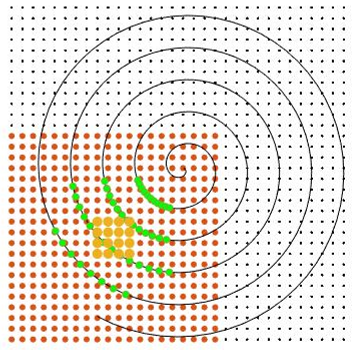
\includegraphics[width=6cm]{kspace_PTX_Patch}
	\caption{\textcolor{red}{WAG: I think you should make two subfigures here: one that illustrates a single target location, and one that illustrates a patch of target locations. Also you should annotate the different widths, in the figures, with arrows. Also add a legend for the dots} 
	Illustration of one instance within the palatalization of a 2D k-space domain design problem. The totally design problem is divided into patches of width 4 cycle/FOV, and the 16 yellow points are the target points in this instance. With inclusion width of 4 cycle/FOV, the 46 green excitation trajectory points within the 12 cycle/FOV wide green square (4 cycle/FOV extended outside of the patch) are considered in this instance. The excitation within the 20 cycle/FOV wide red patch is constrained to zero except the point where the delta function is.}
	\label{fig:Patch}
\end{figure}
An example of this concept is shown in Figure \ref{fig:Patch}. For simplicity of visualization, it is demonstrated in a 2D problem, but the concept is easily extended to 3D. The figure depicts the solution of the $\mathbf{W}$ matrix 16 columns at a time, whose corresponding delta functions live within a patch of width 4 cycle/FOV (yellow points in Figure \ref{fig:Patch}). In this instance where the inclusion width is also 4 cycle/FOV, we truncate the $B_1^+$ map Fourier transforms to zero outside a 4 by 4 cycle/FOV square centered at DC. As a result, we must consider all the excitation trajectory points within a 12 by 12 cycle/FOV square, which is 4 cycle/FOV extended outside of the patch width 4 square, since they may contribute energy to the target locations corresponding to the 16 $\mathbf{W}$ matrix columns. For a single instance of the 16-point target patch shown in Figure \ref{fig:Patch}, the 46 green points on the excitation trajectory may contribute significant energy and are considered in the weight design. Furthermore, we must constrain the total excitation to zero at all k-space locations within a 20 by 20 cycle/FOV red patch in Figure \ref{fig:Patch}. This is because any energy deposited at each considered excitation trajectory points will affect not only the target points in the yellow square, but also the whole 2$\times$4 wide patch around that trajectory point. And the 20 by 20 cycle/FOV red patch is the total of the points that can be affected by all the excitation trajectory points considered in this instance. Therefore, in the solution for this instance, $\mathbf{w}$ is a 46$N_c\times$16 matrix, $\mathbf{S}$ is a 400$N_c\times$46$N_c$ matrix, $\mathbf{S}^{H}\mathbf{S}$ is a 46$N_c\times$46$N_c$ matrix, and $\mathbf{s}_i^{H}$ is a 46$N_c\times$16 matrix. 
%Since $\mathbf{s}_i^{H}$ is no longer related to the $i$th row of $\mathbf{S}$ and $i$th column of $\mathbf{W}$ only, it will be denoted as $\mathbf{S_{targ}}$ in later discussions. 
In the next instance, another 16 columns centered around another 4 points by 4 points patch will be solved. It should be noted that in different instances, the number of neighboring excitation trajectory points (the 46 green points in the previous instance) can vary. We will denote this number of points by $N_n$. $N_n$ can be zero when a patch is at the corners where no excitation trajectory point is adjacent. 
%For patches near edges of the excitation k-space FOV, the solution neighborhood and area may wrap back in a circulant shift fashion, depending on the resolution of the final spatial grid on which the user will evaluate the pulse. In Figure \ref{fig:Patch}), denoted by the red area to the right of Figure \ref{fig:Patch}).

\par The patch width determines the total number of instances to be solved. The inclusion width determines the accuracy of $B_1^+$ information utilized in the design. Together, the patch width and the inclusion width determine how many excitation trajectory points are included in each instance, which further determines the size of $\mathbf{S}^{H}\mathbf{S}$ whose construction is most computationally burdensome within an instance. Therefore, increasing patch width reduces the number of $\mathbf{S}^{H}\mathbf{S}$ matrices to be constructed but increases the burden of constructing each of them. An optimal patch width should be decided case by case for different excitation trajectories. 

\subsection*{Efficient construction of $\mathbf{S}^{H}\mathbf{S}$ matrix}
\par Constructing $\mathbf{S}^{H}\mathbf{S}$ by finding $\mathbf{S}$ is computationally expensive. As described previously, the $((c-1)N_c+t)$-th column of the  $\mathbf{S}$ matrix, $\mathbf{S}_c(\vec{k}-\vec{k}_t)$, is the k-space sensitivity map of the $c$-th coil $\mathbf{S}_c(\vec{k})$ shifted to excitation k-space trajectory location $\vec{k}_t$. These shifts for each column of $\mathbf{S}$ are achieved by applying a linear phase modulation to the spatial domain $B_1^+$ map, followed by a fast Fourier transform (FFT). This process becomes computationally overwhelming when there are many RF samples, which is often the case. Furthermore, the matrix multiplication between $\mathbf{S}^{H}$ and $\mathbf{S}$ is also computationally intensive due to the large row dimension of $\mathbf{S}$ (400$Nt$ in the above example in Figure \ref{fig:Patch}).  


\par Inspired by a rapid GRAPPA calibration method for arbitrary 2D/3D non-Cartesian trajectories proposed in Ref \cite{luo2019grappa}, we have developed a fast and memory-efficient algorithm to solve this problem. A key innovation of Ref \cite{luo2019grappa} is that the algorithm constructs the Hermitian $\mathbf{S}^{H}\mathbf{S}$ matrix directly by finding each of the matrix's lower triangle elements through interpolation, instead of building the $\mathbf{S}$ matrix explicitly followed by matrix multiplication. Conceptually, each element in the Hermitian matrix $\mathbf{S}^{H}\mathbf{S}$ is the vector sum of two shifted k-space sensitivity maps, which is also one single point of their convolution. With the multiplication property of Fourier transform, this convolution in k-space can be calculated from the Fourier transform of the dot product of the two spatial domain $B_1^+$ maps. For a more detailed derivation, please refer to Ref \cite{luo2019grappa}.
In practice, $\mathbf{S}^{H}\mathbf{S}$ is constructed in the following way. We first represent the $\mathbf{S}^{H}\mathbf{S}$ matrix with block matrices. Each block matrix $\mathbf{S}_i^{H}\mathbf{S}_j$ is of size $N_n$ by $N_n$, and $\mathbf{S}_i$ and $\mathbf{S}_j$ are the columns of $\mathbf{S}$ related to the k-space sensitivity maps of the $i$-th and $j$-th coils respectively.

\begin{equation}\label{eq:SHS_blocks}
\mathbf{S}^{H}\mathbf{S} = 
\begin{pmatrix}
\mathbf{S}_1^{H}\mathbf{S}_1 & \cdots & \mathbf{S}_1^{H}\mathbf{S}_{N_c} \\
\vdots  &  \ddots & \vdots  \\
\mathbf{S}_{N_c}^{H}\mathbf{S}_1 & \cdots & \mathbf{S}_{N_c}^{H}\mathbf{S}_{N_c} 
\end{pmatrix}
\end{equation}

Since $\mathbf{S}^{H}\mathbf{S}$ is Hermitian, we only need to find the values within the lower triangle of the matrix, which are the lower triangle blocks $\mathbf{S}_i^{H}\mathbf{S}_j$ with $i>j$. For a given lower triangle block $\mathbf{S}_i^{H}\mathbf{S}_j$  ($i>j$), all of its elements are interpolated from the densely sampled Fourier transform of the dot product of the spatial domain $B_1^+$ maps of the $i$-th and $j$-th coils. The $(m,n)$-th element is the value interpolated at $(\vec{k}_m-\vec{k}_n)$ away from DC. Therefore, to solve all the columns of $\mathbf{W}$, the total number of FFT operations needed in this efficient method is only $N_c(N_c+1)/2$, instead of ${N_t}{N_c}$, and the storage size is also much smaller. In addition to the efficiency related to FFT, this algorithm saves a large matrix multiplication between $\mathbf{S}^{H}$ and $\mathbf{S}$ for the solving of every single column of $\mathbf{W}$. 
Although an alternative strategy of determining each column of $\mathbf{S}$ explicitly by interpolating the $N_s$ sample points from unshifted $B_1^+$ Fourier transforms can also reduce the number of FFT operations, it still has the problem of large multiplications between $\mathbf{S}^{H}$ and $\mathbf{S}$ matrices. Furthermore, to calculate each element of $\mathbf{S}^{H}\mathbf{S}$, there are $2N_s$ number of interpolations involved with this sub-optimal strategy. While with the efficient algorithm there is only one interpolation from the densely sampled Fourier Transform of the dot product of two spatial domain $B_1^+$ maps needed. The extra interpolations involved in the sub-optimal strategy would introduce a larger error to $\mathbf{S}^{H}\mathbf{S}$.  

\subsection*{ Off-Resonance correction}
%\par As shown in Equation \ref{eq:SpatialDomainEquation} when we introduced spatial domain design in Chapter \ref{chap:SpatialDesign}, the equation connecting a pTx pulse to its excitation pattern has an off-resonance dependent term 
$e^{\imath \gamma \Delta B_0(\mathbf{x})(t-T)}$. 
In order to model the off-resonance into our k-space domain design, we adapted a fast implementation of the off-resonance compensation with time segmentation approximation and weighted least-squares interpolators \cite{fessler2005toeplitz}. 
By segmenting the RF pulse into multiple segments, this method disentangles the space-and-time dependent phase accrual induced by main field inhomogeneity into either space- or time- dependent terms, and therefore a same system matrix can be applied within each segment. Mathematically, it is
\begin{equation*}
e^{\imath \Delta\omega_j (t_i-T) }\approx\sum_{l=1}^{L} g_{l}(t_i) e^{\imath \theta_{l}(\Delta\omega_j)}
\end{equation*}
where $i=1\dots Nt$ indexes the RF samples, $j=1\dots Ns$ indexes the spatial locations, and $l$ indexes the time segments. The left term is the problematic space-and-time dependent term, with $\Delta\omega_j$ representing the off-resonance at the location-$j$ obtained from a field map and $T$ being the pulse duration. $g_{il}=b_{l}(t_i)$ are the time-dependent-only weights called temporal interpolators applied upon RF samples. $h_{lj}=e^{\imath \theta_{l}(\Delta\omega_j)}$ are the space-dependent-only phase accrual called spatial interpolators, applied upon the excitation pattern of each weighted RF segment. Therefore, the spatial domain formulation becomes
\begin{equation*}
\mathbf{d}=\sum_{l=1}^{L}diag\{\mathbf{h}_l\}\mathbf{A}(diag\{\mathbf{g}_l\}\mathbf{b})
\end{equation*}
The spatial interpolators can be absorbed into the sensitivity maps. The $\mathbf{S}$ matrix in Equation \ref{eq:MatrixForm} will then become 
\begin{equation*}
\mathbf{S_{offres}}=\sum_{l=1}^{L}\mathbf{S}_l diag\{\mathbf{g}_l\}
\end{equation*}
where the columns of the $\mathbf{S}_l$ matrix, instead of being the aforementioned k-space sensitivity maps, are now the Fourier transform of the dot products of the spatial $B_1^+$ maps and the spatial interpolatros of the $l$-th segment, shifted to corresponding excitation k-space locations. 
The efficient construction of $\mathbf{S_{offres}}^{H}\mathbf{S_{offres}}$ follows the same concept mentioned before. 
But with off-resonance, for the elements within an element matrix $\mathbf{S}_i^{H}\mathbf{S}_j$ in Equation \ref{eq:SHS_blocks}, instead of being interpolated from one densely sampled Fourier transform map, which is of the dot product of the spatial domain $B_1^+$ maps of the $i$-th and $j$-th coils, now they are interpolated from $L(L+1)/2$ different Fourier transform maps, each of which has underlying spatial $B_1^+$ maps with two sets of spatial interpolators absorbed into them. For the $(m,n)$-th element within the element matrix $\mathbf{S}_i^{H}\mathbf{S}_j$, the $L(L+1)/2$ interpolated values were then summed with weights $g_{l_i}(t_m)g_{l_j}(t_n)$, where $l_i$ and $l_j$ are the two segment numbers of the spatial interpolators observed into the corresponding $B_1^+$ maps. 
Compared to the efficient construction method without off-resonance, taking off-resonance into account increases the total number of FFT operations form $N_c(N_c+1)/2$ to $N_cL(N_cL+1)/2$, and increased the number of interpolations needed for each element from 1 to $L(L+1)/2$.  


